\documentclass[a4j, twocolumn, dvipdfmx]{jsarticle}

\usepackage[a4paper, left=2.0cm, right=2.0cm, top=2.0cm, bottom=2.0cm]{geometry}
\usepackage{amsmath}
\usepackage[dvipdfmx]{graphicx}
\usepackage{booktabs}
\usepackage{titlesec}
\usepackage{enumitem}
\usepackage{float}
\usepackage{flushend}
\usepackage{xcolor}
\usepackage{framed}

\titleformat{\section}[block]
  {\normalfont\large\bfseries}
  {\thesection}{0.7em}{}

\titleformat{\subsection}[block]
  {\normalfont\normalsize\bfseries}
  {\thesubsection}{0.7em}{}

\titlespacing*{\section}
  {0pt}{1.5ex plus 0.5ex minus 0.2ex}{0.8ex}

\titlespacing*{\subsection}
  {0pt}{1.2ex plus 0.4ex minus 0.2ex}{0.6ex}

\setlist[itemize]{topsep=4pt, itemsep=2pt, leftmargin=*}

\definecolor{okgreen}{RGB}{30,110,30}
\definecolor{warnred}{RGB}{160,30,30}

\newcommand{\okmark}{\textcolor{okgreen}{\textbf{一致}}}
\newcommand{\halfmark}{\textcolor{black}{\textbf{部分的に一致}}}
\newcommand{\ngmark}{\textcolor{warnred}{\textbf{不一致}}}

\title{
Fang et al. (2020) と本実験の対応関係の検証レポート
}
\author{3CDA2216 笠原秀星}
\date{\today}

\begin{document}
\maketitle

\begin{framed}
\noindent\textbf{結論（先に要約）}\\[2pt]
本実験は，Fang ら\cite{fang2020local}が指摘した以下の\textbf{3つの定性的傾向}については，本実験でも一貫して再現されており，\okmark{}対応づけられる（正しいと言える）。
\begin{enumerate}[leftmargin=1.4em]
  \item 悪性クライアント割合が増えるほど精度が悪化する
  \item Non-IID環境はIID環境より精度が悪化する
  \item 集約手法の中でKrumが最も脆弱である
\end{enumerate}
一方，Fangらの論文中の数値（Table 2(b) など）と本実験のError Rateを\textbf{直接突き合わせて「数値として合っている／間違っている」を判定することはできない}。\ngmark{}
理由は，モデル構造・学習ラウンド数・Non-IIDの生成方式など，実験条件そのものが複数の点で異なっており，数値のギャップがどこから来ているのか（攻撃実装の弱さか，条件の違いか）を切り分けられないためである。詳細は\S 2, \S 4で述べる。
\end{framed}

\section{比較の目的と方法}

本レポートは，卒業論文\texttt{sotsuron.tex}で報告した実験結果が，Fang ら\cite{fang2020local}の論文「Local Model Poisoning Attacks to Byzantine-Robust Federated Learning」（USENIX Security 2020）が示す主張と対応しているかどうかを，(1) 実験条件そのものの対応関係，(2) 攻撃アルゴリズムの実装レベルでの対応関係，(3) 得られた数値の比較，の3段階で検証する。

なお本レポートは\texttt{sotsuron.tex}本体には反映していない独立の検証資料であり，卒論の記述内容を変更するものではない。

\section{実験条件の対応表}

表\ref{tab:setting_correspondence}に，Fangらの論文本文（4.1節，Table 1，Table 7a）および本実験のソースコード（\texttt{pytorchexample/task.py}，\texttt{pyproject.toml}，\texttt{run\_experiments.py}）を直接確認した上での対応関係を示す。

\begin{table*}[t]
\centering
\caption{実験条件の対応関係（Fang et al. 2020 本文・Table 1・Table 7a と，本実験のソースコードを直接確認した結果）}
\label{tab:setting_correspondence}
\footnotesize
\setlength{\tabcolsep}{4pt}
\renewcommand{\arraystretch}{1.15}
\begin{tabular}{@{} p{2.3cm} p{6.5cm} p{5.8cm} c @{}}
\toprule
項目 & Fang et al. (2020) & 本実験 & 判定 \\
\midrule
データセット & MNIST（60k/10k） & MNIST（60k/10k，同一） & \okmark \\
ワーカ数 $m$ & 100（デフォルト） & 100 & \okmark \\
悪性クライアント数 $c$ & 20（デフォルト，20\%） & Malicious Ratio 0.2（20/100） & \okmark \\
評価対象の集約手法 & Krum, Bulyan, Trimmed Mean, Median & FedAvg, Median, Trimmed Mean, Krum, Bulyan & \okmark \\
評価指標 & Testing Error Rate（held-out test set） & Accuracy（held-out test set，$1-$Acc.で比較可） & \okmark \\
Bulyanのロバスト性条件 & $c \leq \frac{m-3}{4}$ & $n \geq 4f+3$ を根拠にRatio 0.3を除外 & \okmark \\
攻撃者の知識 & Full knowledge（全ワーカのローカルモデルを把握） & サーバ側で全クライアント更新を参照して模擬 & \okmark \\
\midrule
モデル構造（``DNN''） & \textbf{CNN}：Conv(3$\times$3$\times$30)+Pool, Conv(3$\times$3$\times$50)+Pool, FC(200), Softmax（Table 7a） & \textbf{全結合MLP}：784$\to$128$\to$64$\to$10（\texttt{task.py}） & \ngmark \\
学習の反復回数 & 2{,}000 iterations（DNN分類器） & 20 rounds（\texttt{NUM\_SERVER\_ROUNDS=20}） & \ngmark \\
Non-IIDの生成方式 & ラベル$l$を対応クライアント群へ確率$p{=}0.5$で割当 & Dirichlet($\alpha{=}0.6$)によるクラスごとの配分（\texttt{task.py}） & \ngmark \\
最適化手法 & 明記なし（SGDが前提の記述） & AdamW，lr$=$0.001（\texttt{task.py}） & \halfmark \\
バッチサイズ & 32（Fashion-MNISTのみ64） & 25 & \halfmark \\
ローカルエポック数 & 明記なし & 1 & (対象外) \\
\bottomrule
\end{tabular}
\end{table*}

表\ref{tab:setting_correspondence}が示す通り，「攻撃者の割合」「対象データセット」「評価指標」「評価対象の集約手法群」といった\textbf{実験の骨格}は正しく対応づけられている。一方で，\textbf{モデル構造・反復回数・Non-IIDの生成方式}という，攻撃の効きやすさに直接影響しうる3つの要素は，Fangらの設定と明確に異なっている。特にモデル構造については，Fangらが``DNN''と呼んでいるものは実際にはCNN（畳み込み層を含む）であり，本実験の全結合MLPとは異なるアーキテクチャである点は，卒論本文中に明記されていなかった重要な相違点である。

\section{攻撃アルゴリズムの対応関係}

\texttt{attack.py}の実装を，Fangらの論文3.2〜3.4節の攻撃定式化と照合した結果を以下に示す。

\subsection{Trimmed Mean / Median：構造的に一致}
Fangらは，honestな更新の座標ごとの最大値・最小値（$w_{max,j}$，$w_{min,j}$）よりさらに外側の値を悪性クライアントへ割り当てる境界値攻撃が理論上最適であることを示している（3.3節）．本実験の\texttt{\_craft\_trimmed\_mean\_median\_attack}も同一の考え方に基づき，攻撃方向に応じて$w_{max}$の外側／$w_{min}$の外側へ値を割り当てている．悪性クライアントごとに押し出し量を段階的にずらす（stagger）実装は，Fangらの論文には明記されていない本実験独自の工夫だが，「座標ごとのtrim処理で悪性値がまとめて除外されるのを防ぐ」という目的に対しては論文の主張と矛盾しない拡張であり，\okmark{}\textbf{構造的に一致}していると判断できる．

\subsection{Krum / Bulyan：戦略は一致，基準点が異なる}
Fangらは，$w'_1 = w_{Re} - \lambda s$（$w_{Re}$：直前ラウンドの受信グローバルモデル）とし，Krumが$w'_1$を選ぶ最大の$\lambda$をTheorem 1の理論的上界から二分探索で求める．本実験の\texttt{\_craft\_krum\_attack}も「Krumに選ばれる最大の$\lambda$を指数拡大＋二分探索で求める」という\textbf{探索戦略自体は同一}である．

ただし，crafted pointの基準点が異なる：Fangは$w_{Re}$（受信グローバルモデル）を起点とするのに対し，本実験は honest updateの重心（\texttt{benign\_center}）を起点としている．これはコード内コメントに明記された意図的な設計変更であり，「honestクラスタが1ラウンドの学習でグローバルモデルから既に離れている場合に，$w_{Re}$起点では$\lambda=0$でも選ばれなくなる」ことを避けるための工夫である．この変更が攻撃を強める方向・弱める方向のどちらに作用するかは解析的には自明ではなく，\halfmark{}\textbf{戦略は同じだが数式は同一ではない}．

\section{数値の比較（参考情報）}

上記の通り実験条件に複数の相違点があるため，以下に示す数値比較は\textbf{攻撃実装の正しさを検証する根拠にはならない}．あくまで「オーダーとしてどの程度離れているか」を確認するための参考情報として提示する．

\begin{figure*}[t]
    \centering
    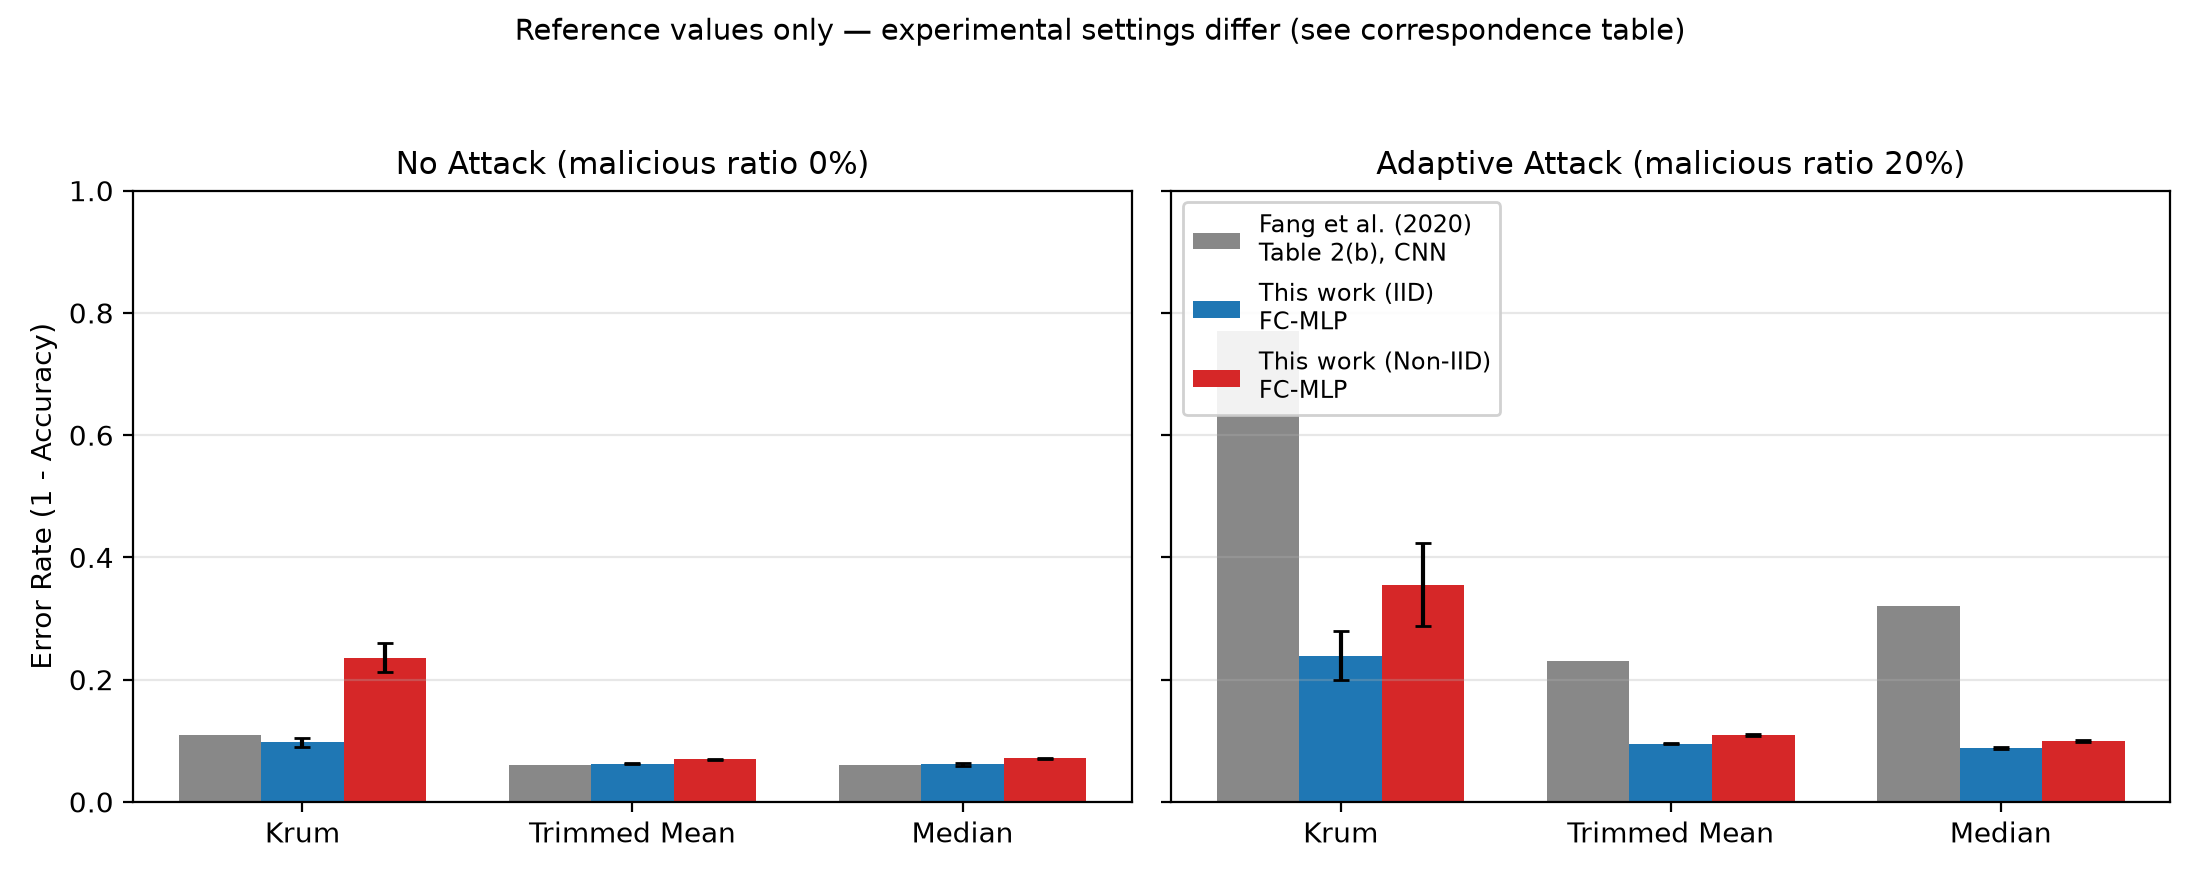
\includegraphics[width=0.85\textwidth]{assets/fang_comparison_error_rate.png}
    \caption{Fang et al. (2020) Table 2(b)（CNN，MNIST，悪性クライアント20\%，Full knowledge攻撃）と，本実験（Malicious Ratio 0.2，Round 20，Seed 1--3平均，誤差棒は標準偏差）のError Rate（$1-$Accuracy）．\textbf{モデル構造・反復回数・Non-IID生成方式が異なるため，この図は数値の優劣を直接判定する根拠にはならない．}}
    \label{fig:fang_comparison}
\end{figure*}

図\ref{fig:fang_comparison}および表\ref{tab:fang_numbers}に示す通り，No Attack時のError Rateは同水準（0.06〜0.24程度）だが，攻撃時のError Rateは本実験の方がFangらの報告値を下回る（特にKrumで約2〜3倍の差）．

\begin{table}[H]
\centering
\caption{Testing Error Rate（$1-$Accuracy）の参考比較．本実験はRound 20・Seed 1--3平均$\pm$標準偏差．}
\label{tab:fang_numbers}
\footnotesize
\begin{tabular}{l cc cc}
\toprule
& \multicolumn{2}{c}{Fang (Table 2b)} & \multicolumn{2}{c}{本実験 IID} \\
\cmidrule(lr){2-3} \cmidrule(lr){4-5}
手法 & No Atk & Full & No Atk & Ratio 0.2 \\
\midrule
Krum & 0.11 & 0.77 & 0.097 & 0.239 \\
Trimmed Mean & 0.06 & 0.23 & 0.063 & 0.096 \\
Median & 0.06 & 0.32 & 0.061 & 0.088 \\
\bottomrule
\end{tabular}

\vspace{4pt}
\begin{tabular}{l cc}
\toprule
& \multicolumn{2}{c}{本実験 Non-IID} \\
\cmidrule(lr){2-3}
手法 & No Atk & Ratio 0.2 \\
\midrule
Krum & 0.236 & 0.355 \\
Trimmed Mean & 0.070 & 0.109 \\
Median & 0.071 & 0.100 \\
\bottomrule
\end{tabular}
\end{table}

この数値差の\textbf{原因を「攻撃実装が弱いから」と断定することはできない}．\S 2で確認した通り，モデル構造（CNN対MLP），反復回数（2,000対20），Non-IID生成方式（確率的グループ割当対Dirichlet）という3つの相違点だけでも，攻撃実装の巧拙とは無関係にこの程度のError Rateの差は生じうるためである．したがって，この表は「本実験の集約手法がFangらの報告より頑健に見える」ことを示す証拠ではなく，\textbf{単純な数値比較が成立しない状況にある}ことを示す証拠として読むべきである．

\section{総合判定}

\begin{itemize}
  \item \textbf{対応づけられる部分（正しいと言える）}：悪性クライアント割合・データセット・評価対象の集約手法・評価指標という実験の骨格はFangらと一致しており，「攻撃者が増えるほど悪化」「Non-IIDの方が悪化」「Krumが最弱」という定性的な3つの結論は，Fangらの主張と正しく対応づけられる．Trimmed Mean / Medianに対する攻撃実装も，理論的な着想のレベルでFangらと構造的に一致している．
  \item \textbf{対応づけられない・不十分な部分}：Fangらの``DNN''は実際にはCNNであり本実験の全結合MLPとは異なる，学習ラウンド数が2桁少ない，Non-IIDの生成方式が異なる，という3つの理由により，\textbf{Error Rateの数値そのものをFangらの論文の数値と直接比較して「合っている／間違っている」と判定することはできない}．Krum/Bulyanに対する攻撃も，探索戦略は同一だが基準点が異なるため，「原論文の数式をそのまま再現した」とは言えない．
\end{itemize}

以上より，本実験は\textbf{Fangらの定性的な主張を再現する検証としては妥当}であるが，\textbf{数値の再現性を主張する根拠としては不十分}である．卒論・発表において両者の数値を並べて提示する場合は，本レポートの表\ref{tab:setting_correspondence}に示した相違点を明記した上で「参考情報」として扱うことを推奨する．

\begin{thebibliography}{9}
\bibitem{fang2020local}
Minghong Fang, Xiaoyu Cao, Jinyuan Jia, Neil Zhenqiang Gong,
``Local Model Poisoning Attacks to Byzantine-Robust Federated Learning,''
Proceedings of the 29th USENIX Security Symposium (USENIX Security 2020),
pp.~1605--1622, 2020.
\end{thebibliography}

\end{document}
